\chapter{R\&D of Gaseous Detectors for Particle Identification}

My Ph.D work starts with the R\&D of two different kinds of gaseous detectors. One is Mini-drift THick Gas Electron Multiplier Chamber (THGEM) used as the readout of Transition Radiation Detector (TRD), the other is Multi-gap Resistive Plate Chamber (MRPC) for Beijing Spectrometer end-cap Time of Flight (eTOF) upgrade. The R\&D motivations and test results of these two gaseous detectors will be discussed in the following sections.

\section{THGEM for TRD}
An Electron Ion Collider (EIC)~\cite{eic} will probe with unprecedented precision the low Bjorken-x domain where gluons and sea quarks dominate for both nucleons and nuclei. A possible realization of the accelerator facility based on RHIC, called eRHIC, has been proposed~\cite{erhic}. The STAR was planned to evolve into eSTAR with a suite of upgrades optimized for the EIC physics program, and the eSTAR detector performance and a broad range of flagship measurements were studied through simulation~\cite{estarloi}. One of the major experimental challenges was to cleanly identify the scattered electron. Thus, a compact TRD located in forward rapidity (-2 $<\eta<$ -1), was proposed~\cite{startrdproposal}. The proposed TRD based on THGEM, provides $dE/dx$ measurement in addition to the transition radiation (TR) signal and tracklet reconstruction capability. The operation principle and design of the THGEM based TRD chamber is depicted by Fig.~\ref{trd_working_principle}. The TRD serves two functions. Firstly, it provides additional $dE/dx$ measurement at the entire momentum range. This is essential for small angle scattering, where only a small section of the particle trajectory falls within the tracking detector acceptance, resulting in few hits in the tracking detector and worse $dE/dx$ resolution (1/$\sqrt{N}$ rule). Through the simulation~\cite{startrdproposal}, TRD with 300 $\mu$m spatial resolution is enough for tracking due to the thick TRD radiator and material in the TPC endcap. Secondly, it adds necessary TR signal to particles at high momentum. The TR threshold is around $\gamma$~$>$~1000$\sim$2000. From a practical standpoint, only electrons provide such radiation into the ionization chamber in the TRD, boosting the effective electron $dE/dx$ to even higher values from the existing relativistic rise.

\begin{figure}[htbp]
\centering
\includegraphics[keepaspectratio,width=0.6\textwidth]{detector/gemTRD_workingPrinciple.png}
\figcaption{Schematic of the THGEM based TRD.}
 \label{trd_working_principle}
\end{figure}

\subsection{The THGEM Chamber}
The THGEM chamber, one of the most recently developed micropattern gas detectors, is a robust, high-gain gaseous electron multiplier, and has a hole-structure~\cite{thgem,thgem1}. It is manufactured economically by mechanically drilling sub-millimeter diameter holes in a thin printed-circuit board (PCB), followed by Cu-etching of the hole's rim.

\begin{figure}[htbp]
\begin{minipage}[htbp]{0.68\linewidth}
\centering
\includegraphics[width=0.9\textwidth]{detector/foil_structure.png}
\caption{The structure of the THGEM foil. \label{foil_structure}}
\end{minipage}
\hfill
\begin{minipage}[htbp]{0.3\linewidth}
\centering
\includegraphics[width=1.0\textwidth]{detector/readout_structure.png} 
\caption{The readout board structure of the THGEM chamber.\label{readout_structure}}
\end{minipage}
\end{figure}

The THGEM chamber in this study uses three THGEM foils in cascade. The foil structure is shown in Fig.~\ref{foil_structure}. The major parameters include foil thickness 300 $\mu$m, hole diameter 150 $\mu$m, and hole pitch 400 $\mu$m. The rim clearance region around the hole is $\sim$50 $\mu$m. The effective readout area given by the foil  is 10$\times$10 cm$^{2}$. Figure~\ref{readout_structure} depicts the readout board structure of the THGEM chamber. The readout unit, with a pitch of 800 $\mu$m, is strip-style in $x$ direction while pad-style (inter-connected beneath) in $y$ direction. The thickness of the THGEM chamber ionization gap is 11.3 mm. The THGEM chamber is placed in a gas-tight aluminum box with a gas mixture (90$\%$ Ar + 10$\%$ CO$_{2}$) at atmospheric pressure.

\subsection{Cosmic Ray Test System Setup}\label{systemsetup}
Two different setups of the cosmic ray test system are shown in Fig.~\ref{cosmic_system_setup}. Three scintillators read out by photomultipliers, providing trigger for this system, are placed upstream and downstream of the three GEM chambers. The system consists of two regular GEM chambers (GEM0, GEM2) and one THGEM chamber (GEM1) in between. The vertical ($z$ direction) distance between the THGEM chamber and the regular GEM chamber is 10.5 cm. The readout boards of the two regular GEM chambers, with 3.8 mm ionization gap width, are identical to that of  the THGEM chamber. These two GEM chambers are used to calibrate the THGEM chamber. They can also be used to measure the cosmic ray tracklet slope to study the track reconstruction capability of the THGEM chamber. The left setup in Fig.~\ref{cosmic_system_setup} with all the detectors aligned vertically is used to measure the detection efficiency of the THGEM chamber while the right setup with 4.1 cm horizontal offset between the THGEM chamber and the regular GEM chamber along $y$ direction is used to study other performance of the THGEM chamber, such as spatial resolution, track reconstruction capability,  gain uniformity and stability. The front end electronics (FEE) of these three GEM chambers are all based on the APV25-S1 chip~\cite{apv}, and the readout system is almost the same as that of the forward GEM tracker (FGT) at the STAR experiment~\cite{fgtreadout}. The only difference is that the front end card has only 2 APV chips rather than 5 used for the FGT. Each readout unit is sampled in 27 time bins (26.7 ns bin width) along electron drift direction ($z$ direction).

\begin{figure}[htbp]
\centering
\includegraphics[keepaspectratio,angle=270,width=1.0\textwidth]{detector/cosmic_system_setup.pdf}
\figcaption{Schematic of the two different setups of the cosmic ray test system. Left Panel: The setup with the THGEM chamber (GEM1) and two regular GEM chambers (GEM0, GEM2) aligned vertically. Right Panel: The setup with 4.1 cm horizontal offset between the THGEM chamber and the regular GEM chamber along $y$ direction. The distance between the THGEM chamber and the regular GEM chamber along $z$ direction is 10.5 cm.}
 \label{cosmic_system_setup}
\end{figure}

\subsection{Performance of The THGEM Chamber}
\paragraph{Efficiency plateau} 
The detection efficiency is scanned as a function of HV with the cosmic ray test system to obtain the optimum operating voltage of the THGEM chamber. The efficiency plateau of the THGEM chamber is shown in Fig.~\ref{eff_plateau}. The detection efficiency goes above 90$\%$ when the applied HV is higher than -3.5 kV. -3.65 kV is selected as the operating HV for the THGEM chamber at which the efficiency is greater than 94$\%$.

\paragraph{Spatial resolution} 
The performance of the two regular GEM chambers was tested elsewhere before this cosmic ray test. Their spatial resolutions are found to be better than 150 $\mu$m. The vertically incident cosmic ray tracks (tan$\theta$ $<$ 0.1, $\theta$ is the zenith angle) are selected to measure the spatial resolution of the THGEM chamber. Figure~\ref{thgem_spatial} shows the residual distribution in the $x$ direction, $x_{project}-x_{measure}$, where $x_{project}$ is the cosmic ray trajectory position at the THGEM chamber projected from the two regular GEM chambers and $x_{measure}$ is the hit position measured by the THGEM chamber. The residual distribution in $y$ direction is very similar. The 1-D spatial resolution of the THGEM chamber is $\sim$220 $\mu$m after subtracting the contribution from the two regular GEM chambers. 
\begin{figure}[htbp]
\begin{minipage}[htbp]{0.48\linewidth}
\centering
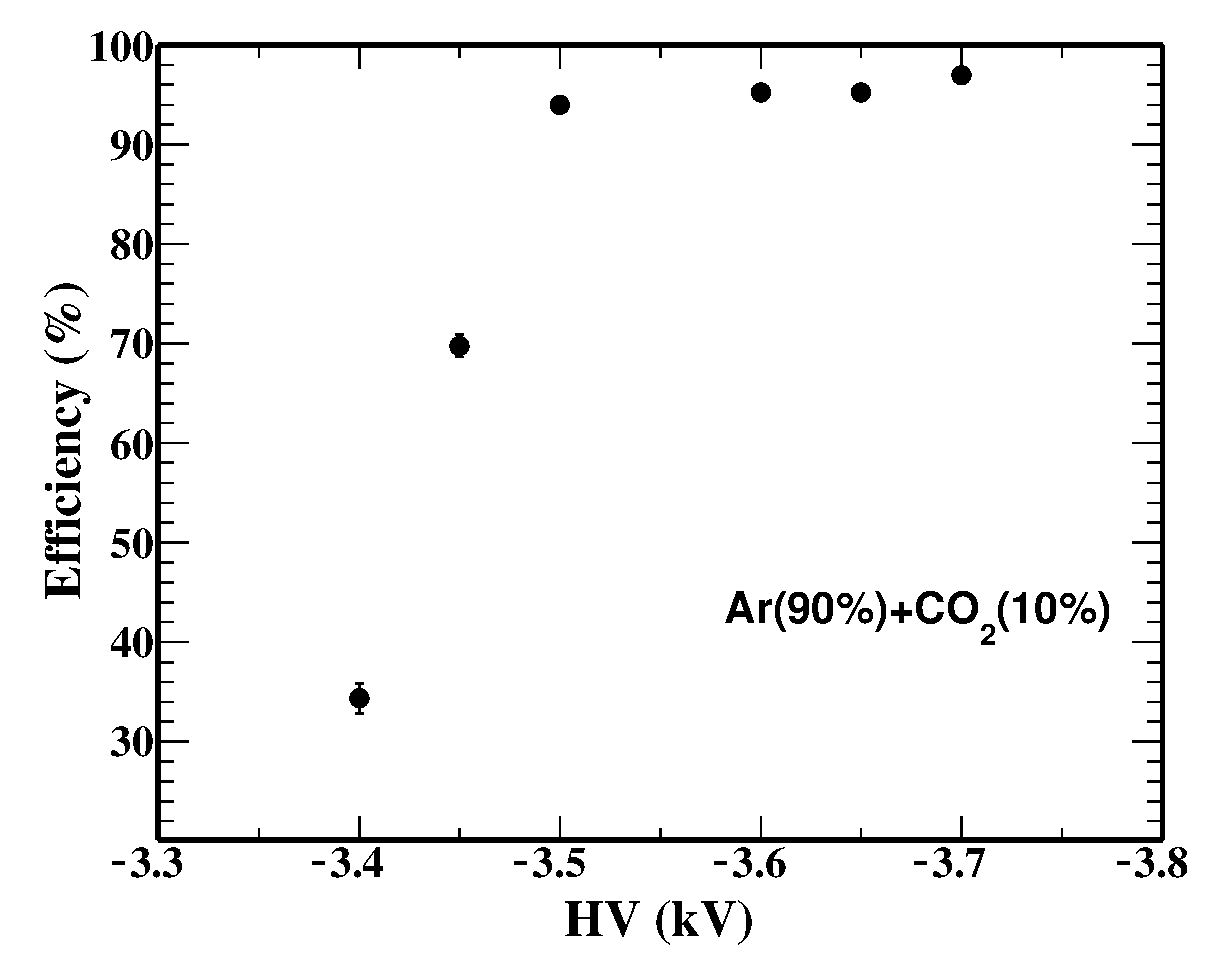
\includegraphics[width=1.0\textwidth]{detector/eff_vs_hv.eps}
\caption{The efficiency plateau of the THGEM chamber. \label{eff_plateau}}
\end{minipage}
\hfill
\begin{minipage}[htbp]{0.5\linewidth}
\centering
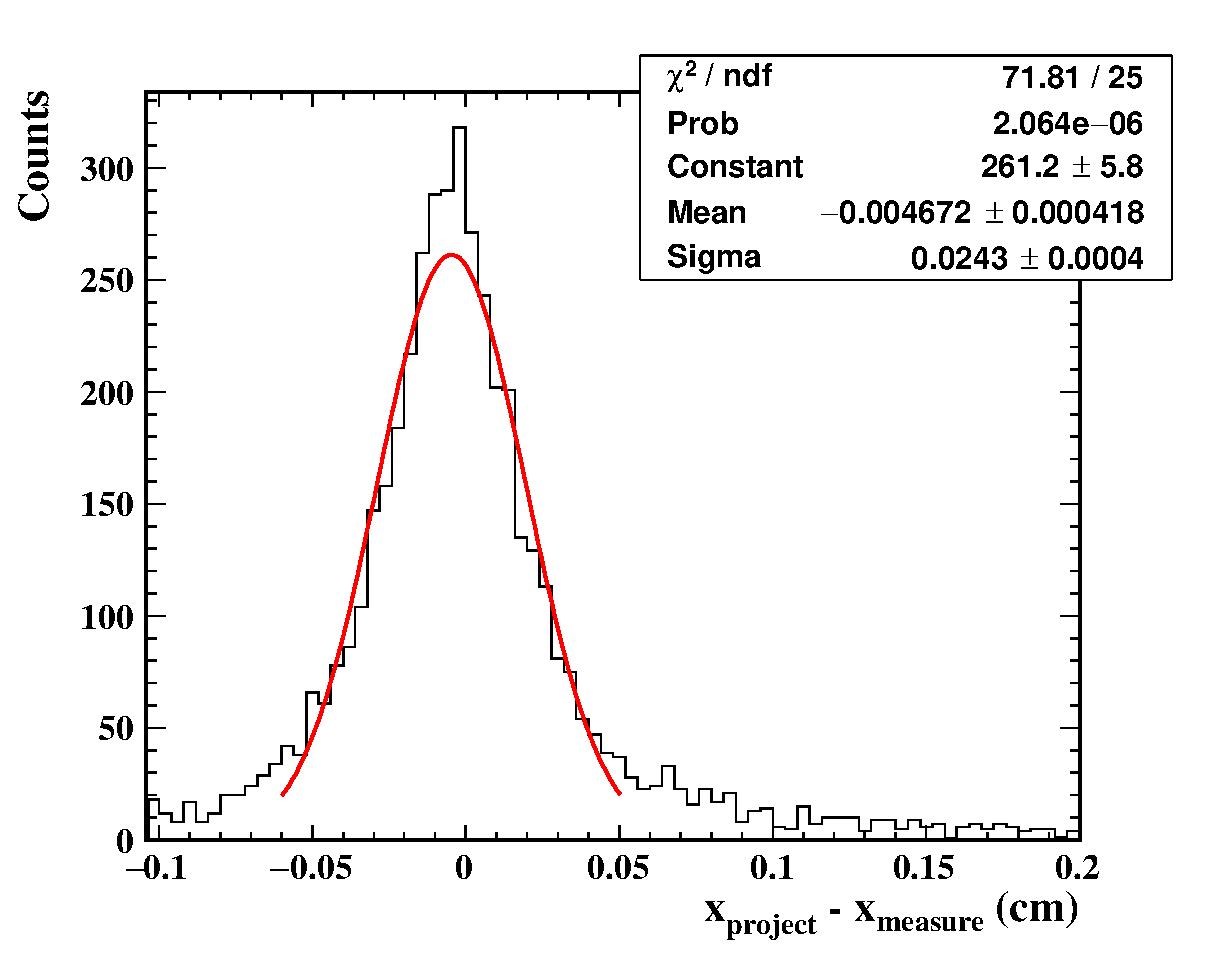
\includegraphics[width=1.0\textwidth]{detector/spatial_resolution.eps} 
\caption{The residual distribution in $x$ direction.\label{thgem_spatial}}
\end{minipage}
\end{figure}

\paragraph{Electron drift velocity} 
The electron drift velocity in the gas mixture can be obtained through correlating the hit point's 
 $z$ position with its corresponding drift time in the THGEM chamber. The hit point with maximum energy deposit of a large zenith angle track is selected firstly. The $x$, $y$ positions ($x_{1}$, $y_{1}$) of this point are calculated by the center of gravity method. The $z$ position ($z_{1}$) of this point is then derived through the equation  $ \frac{\sqrt{(x_{0}-x_{2})^{2}+(y_{0}-y_{2})^{2}}}{|z_{0}-z_{2}|} = \frac{\sqrt{(x_{0}-x_{1})^{2}+(y_{0}-y_{1})^{2}}}{|z_{0}-z_{1}|}$,  where $x_{0}$, $y_{0}$ are the $x$, $y$ positions measured by GEM0 using the center of gravity method while $x_{2}$, $y_{2}$ are provided by GEM2. $z_{0}$, $z_{2}$ are the positions of GEM0 and GEM2 along $z$ direction. This process is depicted in Fig.~\ref{driftv_principle}. The correlation between $z$ position and its corresponding drift time is shown in Fig.~\ref{thgem_v}(a). The electron drift velocity can then be extracted from a linear fit to the correlation. The electron drift velocity (at drift E $\approx$ 0.26 kV/cm) obtained using this method is 2.26 cm/$\mu$s, consistent with the data commonly used in the literature~\cite{driftv_data}. The spatial resolution of the THGEM chamber in $z$ direction can be derived by plotting the difference of $z$ position projected by two regular GEM chambers and the $z$ position calculated from the drift velocity and drift time. The overall spatial resolution in $z$ direction is $\sim$1.1 mm, as Fig.~\ref{thgem_v}(b) depicts, including the uncertainty from the trigger clock distribution (TCD) ($\sim$0.2 mm) and the uncertainty from the THGEM and the regular GEM chamber spatial resolutions in $x$, $y$ direction ($\sim$0.8 mm, $\frac{\sqrt{\sigma_{x_{0}}^{2}+\sigma_{x_{1}}^{2}}}{tan\theta}$, this formula is derived under the assumption that the THGEM (GEM) chamber has the same spatial resolution in $x$, $y$ direction. $\sigma_{x_{0}}$ = 0.15 mm is the regular GEM chamber spatial resolution in $x$ direction while $\sigma_{x_{1}}$ = 0.22 mm is the THGEM chamber spatial resolution in $x$ direction.  and the average tan$\theta$ of the collected cosmic ray is 0.32. With these contributions subtracted, the intrinsic spatial resolution in $z$ direction of the THGEM chamber is $\sim$0.7 mm.
 
\begin{figure}[htbp]
\begin{center}
\includegraphics[keepaspectratio,width=0.8\textwidth]{detector/drift_v_principle.png}
\vspace*{-3mm}
\caption{The principle of deriving maximum energy deposit point's z position.} \label{driftv_principle}
\end{center}
\end{figure}
\begin{figure}[htbp]
\begin{center}
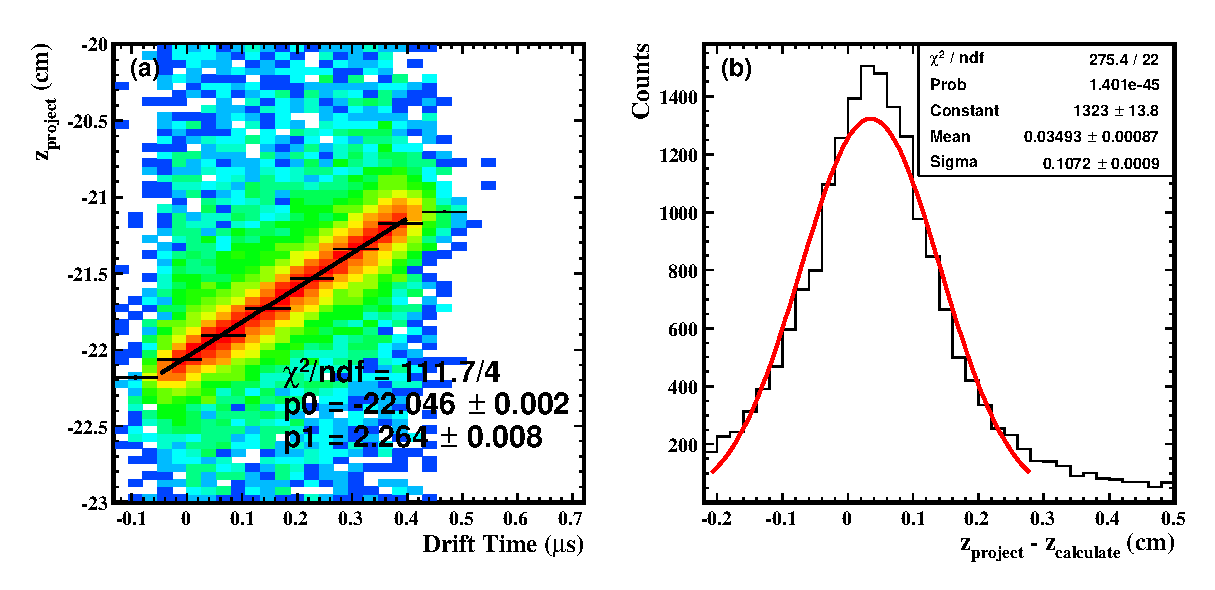
\includegraphics[keepaspectratio,width=1.0\textwidth]{detector/drift_velocity.eps}
\vspace*{-3mm}
\caption{(a) The correlation between $z$ position of the point with maximum energy deposit and its corresponding drift time. (b) The residual distribution of $z$ position, $z_{project}$ is the $z$ position projected by two regular GEM chambers, $z_{calculate}$ is the $z$ position calculated from the drift velocity and drift time.} \label{thgem_v}
\end{center}
\end{figure}

\paragraph{Track reconstruction capability} 
The cosmic ray can be reconstructed just by the THGEM chamber. Firstly, searching for a hit point for each time bucket. If found, the $x$, $y$ positions of this point are calculated using the center of gravity method. Secondly, all these hit points are fitted by a linear function to obtain the cosmic ray tracklet slope (tan$\theta$)  if the number of points is more than two. Thus, the correlation between $slope_{THGEM}$ (measured by the THGEM chamber itself) and $slope_{Two~Regular~GEMs}$ (the slope of the same cosmic ray track measured by the two regular GEM chambers) can be used to study the tracklet slope resolution of the THGEM chamber, which characterizes the track reconstruction capability. The resolution of tracklet slope obtained by the two regular GEM chambers is $\sim$$10^{-3}$ since the distance between the two regular GEMs along $z$ direction is 21.0 cm and the regular GEM's spatial resolution in $x$ or $y$ direction is $\sim$150 $\mu$m. Figure~\ref{track_reconstruction} shows the correlation between tracklet slope measured by the THGEM chamber and that measured by the two regular GEM chambers in $x$ direction, the tracklet slope resolution of the THGEM chamber in $x$ and $y$ direction and the THGEM chamber tracklet slope resolution as a function of cosmic ray incident angle. The tracklet slope resolution in $x$ ($y$) direction is 0.03. Moreover, the results shown in Fig.~\ref{track_reconstruction}(d) indicate that the tracklet slope resolution deteriorates with increasing incident angle as previously observed in similar studies~\cite{spatialResvsAngle}.

\begin{figure}[htbp]
\begin{center}
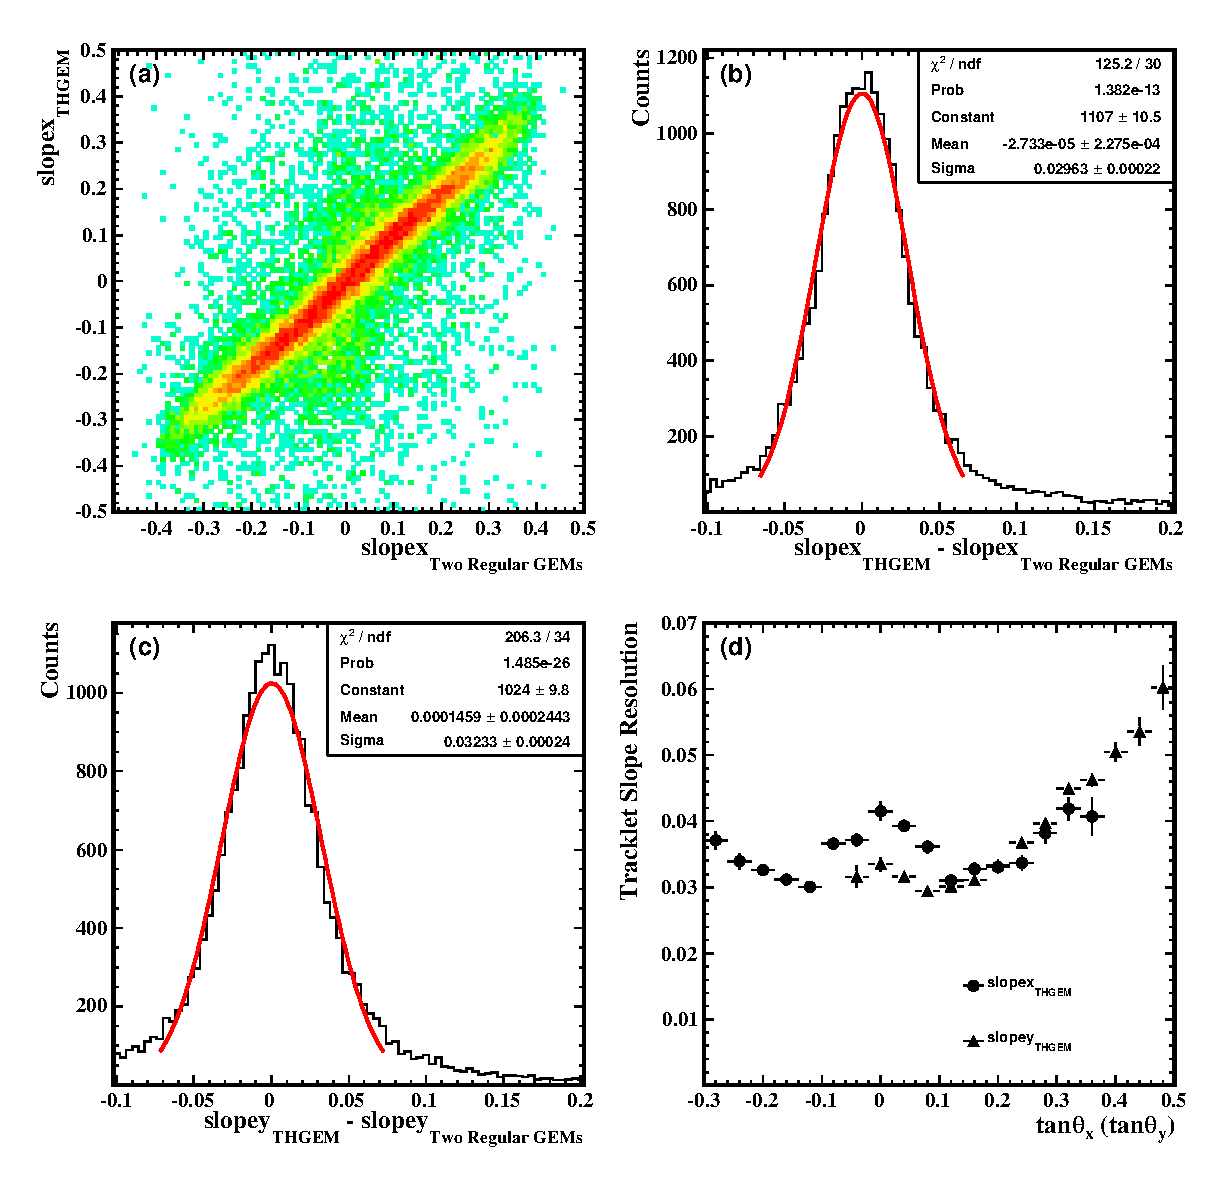
\includegraphics[keepaspectratio,width=0.98\textwidth]{detector/track_reconstruction_capability.eps}
\vspace*{-3mm}
\caption{(a) The correlation between the tracklet slope measured by the THGEM chamber and that measured by the two regular GEM chambers in $x$ direction. (b) The residual distribution of the tracklet slope in $x$ direction. (c) The residual distribution of  the tracklet slope in $y$ direction. (d) The tracklet slope resolution of the THGEM chamber in $x$ or $y$ direction as a function of incident angle.} \label{track_reconstruction}
\end{center}
\end{figure}

\paragraph{Gain uniformity and stability} 
The readout board of the THGEM chamber is artificially divided into 6$\times$6 identical sub-regions. The non-uniformity is described using $\frac{dE/dx-<dE/dx>}{<dE/dx>}$, where $dE/dx$ is the average recorded charge for all tracks passing the given region while $<$$dE/dx$$>$ is the average of  $dE/dx$ over all regions. The measured $dE/dx$ of different sub-regions is shown in Fig.~\ref{foil_uniformity}(a). The $dE/dx$ non-uniformity for most of the sub-regions (32 out of 36) is less than 15$\%$ as Fig.~\ref{foil_uniformity}(b) depicts. The $<$$dE/dx$$>$ as a function of operating time for the THGEM can be found in Fig.~\ref{stability}. The THGEM shows an increase of gain in the first 24 hours and remains stable afterwards.

\begin{figure}[htbp]
\begin{center}
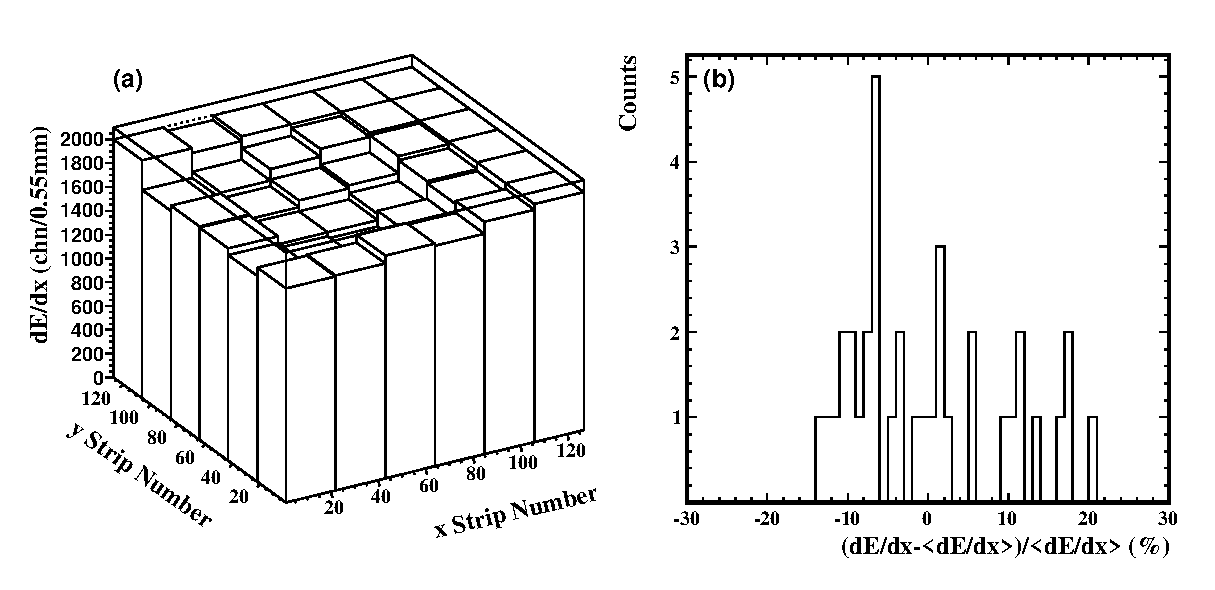
\includegraphics[keepaspectratio,width=1.0\textwidth]{detector/foil_uniformity.eps}
\vspace*{-3mm}
\caption{(a) $dE/dx$ value of each sub-region, $dE/dx$ is the average recorded charge for all tracks passing the given region. (b) $dE/dx$ non-uniformity of each sub-region, $<$$dE/dx$$>$ is the average of $dE/dx$ over all regions.} \label{foil_uniformity}
\end{center}
\end{figure}

\begin{figure}[htbp]
\begin{center}
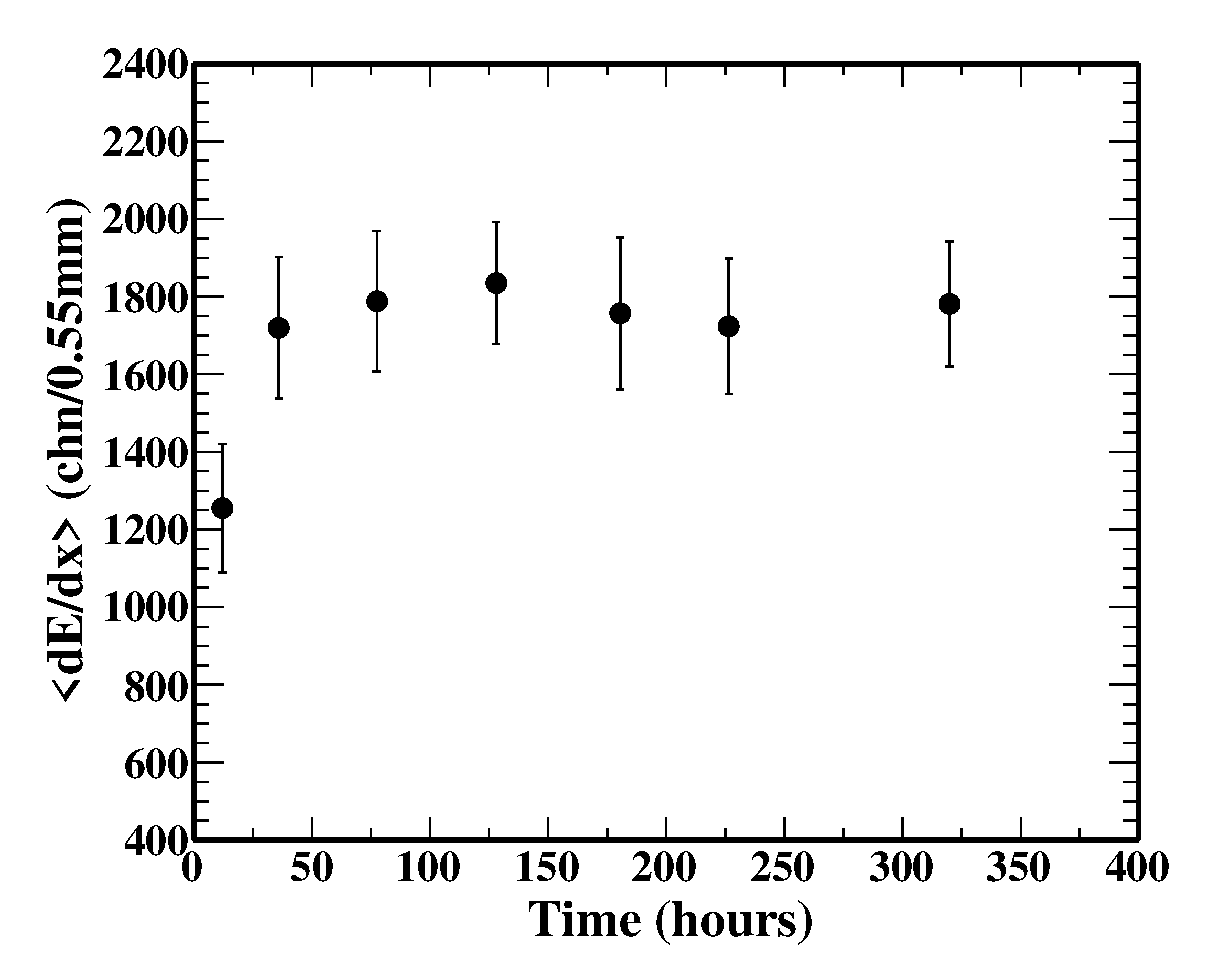
\includegraphics[keepaspectratio,width=0.5\textwidth]{detector/gain_vs_time.eps}
\vspace*{-3mm}
\caption{The $<$$dE/dx$$>$ as a function of  operating time for the THGEM chamber.} \label{stability}
\end{center}
\end{figure}

\subsection{Summary of The THGEM Cosmic Ray Test}
The results of the cosmic ray test reveal the excellent performance of the THGEM chamber. The detection efficiency of the THGEM chamber is greater than 94$\%$ and the 1-D spatial resolution is $\sim$220 $\mu$m. Moreover, the THGEM chamber shows good spatial resolution ($\sim$0.7 mm) along electron drift direction and good tracklet slope resolution (0.03) in $x$, $y$ direction, which are important for the small incident angle track reconstruction. In addition to these, the THGEM chamber shows good uniformity and stability during a long run. Such work offers an important reference for the proposed TRD design.

\section{MRPC for Beijing Spectrometer eTOF Upgrade}
The Beijing Spectrometer~\cite{beijingSpe} is a general-purpose detector designed for $e^{+}e^{-}$ collisions in the $\tau$-charm energy region at the Beijing Electron Positron Collider (BEPC\uppercase\expandafter{\romannumeral2}). The old eTOF of Beijing Spectrometer consisted of 2$\times$48 fast scintillators readout with fine-mesh photomultiplier tubes~\cite{oldETOF}. The time resolution was 110 ps for muons in the di-$\mu$ events, 138 ps for pions, and 148 ps for electrons in the Bhabha events. The momentum range for $K/\pi$ separation (2$\sigma$) was limited to 1.1 GeV/$c$~\cite{pikIdentification}. A GEANT4 simulation was carried out~\cite{eTOFSimulation} to study the cause of the degradation of time resolution for electrons. The major reason was found to be the multiple scattering effects upon materials ($\sim$0.28 $X_{0}$) between the main drift chamber (MDC) end-cap and the eTOF. Despite the low event multiplicities (<4 tracks per event), the secondary particles produced eTOF upstream (mainly gammas, electrons and positrons) caused a high multi-hit probability for electron events (around 71.5\%) in each eTOF scintillator module, making the position-dependent time calibration difficult. A new particle detection technique insensitive to gamma and a smaller readout cell size are thus required for the eTOF upgrade. The MRPC~\cite{mrpc0,mrpc1,mrpc2}, with good time resolution, high detection efficiency and relatively low cost, can be produced with high granularity and is relatively insensitive to gamma. A proposal was raised in 2010 to upgrade the Beijing Spectrometer eTOF with the MRPC technology, aiming at an overall 80 ps time resolution for minimum ionizing particles (MIPs), which will extend the momentum range for $K/\pi$ separation (2$\sigma$) to 1.4 GeV/$c$.

\subsection{The MRPC Modules}
Three MRPC prototypes with different readout modes were manufactured. The length of each MRPC module is 35.2 cm while the widths are shown in Fig.~\ref{mrpcView0}. Two readout modes, namely single-end and double-end, are considered. The single-end readout MRPC consists of 2$\times$12 readout cells. The lengths of the cells range from 4.1 cm to 6.8 cm. The double-end readout MRPC has 12 readout cells with the lengths ranging from 8.6 cm to 14.1 cm. The interval between any adjacent cells is 4mm. Among the three modules tested, two have single-end readouts and one has double-end readouts. Figure~\ref{mrpcView1} schematically shows a cross-sectional view of the MRPC prototypes. All the MRPC prototype modules have 12 gas gaps arranged in a double-stack configuration mirrored with respect to the central electrode. The gap width is 220 $\mu$m, defined by nylon fishing line. Floating glass sheets with volume resistance of ~$10^{13}$ $\Omega\cdot$cm are used as the resistive plates. The thicknesses are 0.4 mm and 0.55 mm for the inner and outer glass, respectively. The outer surfaces of the outermost glass in each stack are coated with graphite tapes, which serve as high voltage electrodes. The surface resistivity of the graphite tape is about 200 k$\Omega$/$\Box$. Two pieces of 3 mm thick honeycomb-board are attached to the outer surfaces of the detector to reduce structural deformations. The MRPC prototype module is placed in a gas-tight aluminum box whose total thickness is 2.5mm (~0.028 $X_{0}$), flushed with a standard gas mixture (90\% Freon + 5\% SF6 + 5\% iso-C$_{4}$H$_{10}$).

\begin{figure}[htbp]
\begin{minipage}[htbp]{0.43\linewidth}
\centering
\includegraphics[width=0.9\textwidth]{detector/mrpc_view0.png}
\caption{The layouts of the two readout patterns (single-end readout (a) and double-end readout (b)) from a top view. \label{mrpcView0}}
\end{minipage}
\hfill
\begin{minipage}[htbp]{0.55\linewidth}
\centering
\includegraphics[width=1.0\textwidth]{detector/mrpc_view1.png} 
\caption{The schematic drawing of the cross-section of the MRPC.\label{mrpcView1}}
\end{minipage}
\end{figure}

\subsection{Beam Test System Setup}
A beam test was performed at the E3 line of BEPC\uppercase\expandafter{\romannumeral2} using the secondary particles (mainly $e^{+/-}$, $\pi^{+/-}$, p) from an incident electron beam hitting a carbon target. The momenta of the secondary particles are around 600 MeV/$c$. Among these secondary particles, protons are dominant. The setup of the beam test is shown in Fig.~\ref{beamtestSetup}. The Cherenkov detector (C0) is used to veto the electron. The MRPC module, placed in a gas-tight aluminum box, is fixed on a movable platform. The differential output signals of the MRPC are fed to the FEE directly. The coincidence signal of two larger scintillators (S1, S2) and four smaller scintillators (T1-4) is used as the trigger of the beam test DAQ system. Meanwhile, the four smaller scintillators (2$\times$5 cm$^{2}$ active area) both provide a reference time (T$_{0}$) for the MRPC module, and identify the incident particle species through their charge spectra. The signals from the T$_{0}$, after discrimination and LVDS conversion, are sent to the TDIG for a leading-edge time measurement. The charges of the T$_{0}$ signals are measured by a charge-to-digital converter (QDC) module after proper delay. The logic diagram of the beam test DAQ system is shown in Fig.~\ref{daqSys}.

\begin{figure}[htbp]
\begin{center}
\includegraphics[keepaspectratio,width=0.8\textwidth]{detector/beamtest_setup.png}
\vspace*{-3mm}
\caption{The setup of beam test experiment.} \label{beamtestSetup}
\end{center}
\end{figure}

\begin{figure}[htbp]
\begin{center}
\includegraphics[keepaspectratio,width=1.0\textwidth]{detector/daq_logic.png}
\vspace*{-3mm}
\caption{The logic diagram of the beam test DAQ system.} \label{daqSys}
\end{center}
\end{figure}

\subsection{Performance of The MRPC Modules}

\paragraph{The HV Scan}
The efficiency and time resolution are scanned as a function of the high voltage (HV) in order to find the optimum operation voltage of the MRPC. The MRPC efficiency plateau and time resolution of the two different readout modes are shown in Fig~\ref{eff_res}. For the single-end readout mode, the detection efficiency is above 98\% when the applied HV is higher than $\pm$5.8 kV for protons and $\pm$6.6 kV for pions (MIP). To keep the efficiency of the double-end readout MRPC above 98\%, the applied HV has to be greater than $\pm$6.4 kV and $\pm$7.0 kV for protons and pions, respectively. Comparing the two different readout modes, it is clear that the double-end readout MRPC needs higher working HV to achieve better time resolution. This is understood since each end of the double-end readout MRPC cell shares the induced signal charge almost equally. For the results reported in following sections, the corresponding working HVs are ±7.0 kV and ±7.2 kV for the single-end and double-end readout MRPC, respectively.

\begin{figure}[htbp]
\begin{center}
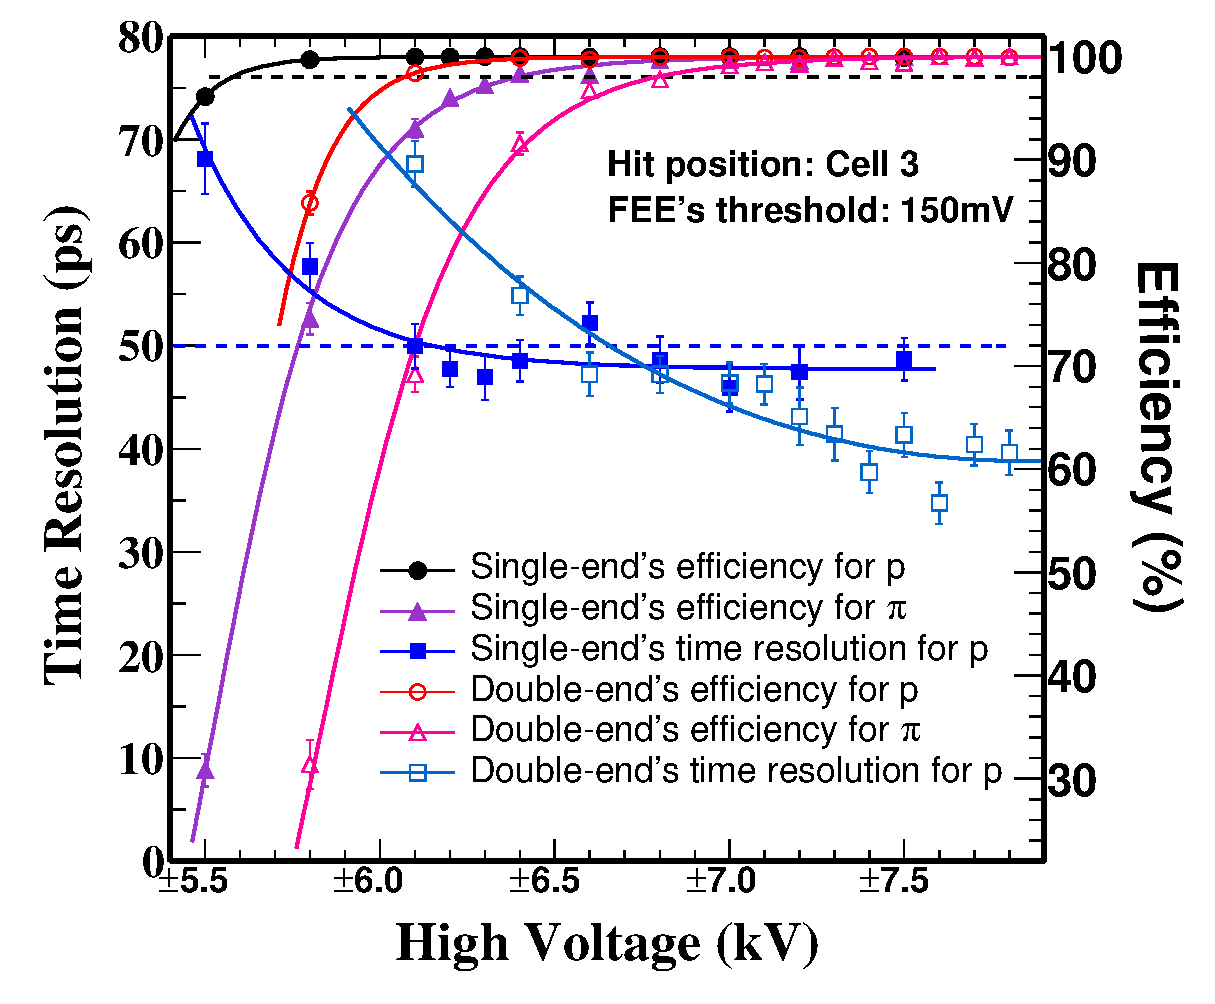
\includegraphics[keepaspectratio,width=0.66\textwidth]{detector/eff_res_vs_hv.eps}
\vspace*{-3mm}
\caption{The HV dependence of the efficiency and time resolution of two different readout MRPCs.} \label{eff_res}
\end{center}
\end{figure}

\paragraph{The Beam Position Scan Across The Cells}
Since the MRPC modules are made in trapezium shape, the length of each cell varies. Scans across the cells are done to investigate the influence of different cell lengths. In the following discussion, the shorter cell starts with the lower cell ID.
For the single-end readout mode, two identical MRPC modules were placed close to each other and tested at the same time. The one upstream is defined as MRPC1, the other one is defined as MRPC2. They have similar performance as shown in Fig.~\ref{single_end_padscan_across}. The time resolution is less than 50 ps for most cells except for the two outmost ones. Similarly, the double-end readout MRPC has also been scanned across the cells. The overall time resolution is $\sim$40 ps, and the cell length has negligible influence on the time resolution, as shown in Fig.~\ref{double_end_padscan_across}.

\begin{figure}[htbp]
\begin{minipage}[htbp]{0.49\linewidth}
\centering
\includegraphics[width=1.0\textwidth]{detector/single_padscan_across.png}
\caption{The cross-cell scan result of the single-end readout MRPC. \label{single_end_padscan_across}}
\end{minipage}
\hfill
\begin{minipage}[htbp]{0.49\linewidth}
\centering
\includegraphics[width=1.0\textwidth]{detector/double_padscan_across.png} 
\caption{The cross-cell scan result of the double-end readout MRPC.\label{double_end_padscan_across}}
\end{minipage}
\end{figure}

\paragraph{The Beam Position Scan Along The Cells}
To investigate the detector performance with respect to the different particle incident position, especially for the single-end readout mode, a scan has been performed along the cell. Two cells (cell 6 and cell 11) are scanned with 1-cm step. As shown in Fig.~\ref{scanSchedule} and Fig.~\ref{positionScanAlong}, the time resolution seems to be slightly worse when the hits are close to the readout end of the cell where signal is fed out, as previously observed in similar studies~\cite{positionDep}.

\begin{figure}[htbp]
\begin{center}
\includegraphics[keepaspectratio,width=0.8\textwidth]{detector/scan_schedule.png}
\vspace*{-3mm}
\caption{The beam scan positions along the cells of the single-end readout MRPC, with a scan step of 1 cm.} \label{scanSchedule}
\end{center}
\end{figure}

\begin{figure}[htbp]
\begin{center}
\includegraphics[keepaspectratio,width=0.49\textwidth]{detector/single_positionscan_pad6.png}
\includegraphics[keepaspectratio,width=0.49\textwidth]{detector/single_positionscan_pad11.png}
\vspace*{-3mm}
\caption{Scans along the cells of the single-end readout MRPC for (a) cell 6 and (b) cell 11.} \label{positionScanAlong}
\end{center}
\end{figure}

\begin{figure}[htbp]
\begin{center}
\includegraphics[keepaspectratio,width=0.7\textwidth]{detector/BES_eTOF_resolution.png}
\vspace*{-3mm}
\caption{The time resolutions of eTOF MRPC modules, which are obtained from collision data.} \label{eTOFRes}
\end{center}
\end{figure}

\subsection{Summary of The MRPC Beam Test}
The results of the beam test at the BEPC E3 line prove the excellent performance of these MRPC modules. The efficiencies of all three MRPC prototypes are higher than 98\%. The time resolution of the double-end readout MRPC can reach 40 ps for 600 MeV/$c$ protons. After subtracting the contribution from the beam position uncertainty, the intrinsic time resolution of the single-end readout MRPC is expected to be better than 50 ps for MIP. For the double-end readout mode, the incident position has negligible effect on the MRPC performance. According to the results of this beam test, the performance of the double-end readout MRPC is insensitive to the position of
incidence. Since the tracking performance is limited in precision within the Beijing Spectrometer eTOF acceptance, the double-end readout MRPC is a better choice for the Beijing Spectrometer eTOF upgrade according to this beam test. In November 2015, the MRPC-based eTOF system was fully installed in Beijing Spectrometer. The time resolution of the MRPC-based eTOF system obtained from the collision data is $\sim$60 ps, as shown in Fig.~\ref{eTOFRes}.

%封面是按照制本厂的要求制作的,其中行宽和行高都是固定的,中文标题最多占两行,英文标题最多占三行。如果您的题目超过了这个限制,请缩减题目长度,不要擅自修改模板中的相关配置参数。

